
\chapter{Specifikacija programske potpore}

\section{Funkcionalni zahtjevi}

\noindent \textbf{Dionici:}

\begin{packed_enum}
	
	\item Korisnici	
	\item Javnost	
	\item Razvojni tim
	\item Naručitelj
	
\end{packed_enum}

\noindent \textbf{Aktori i njihovi funkcionalni zahtjevi:}


\begin{packed_enum}
	\item  \underbar{Neregistrirani/neprijavljeni korisnik(inicijator) može:}
	
	\begin{packed_enum}
		
		\item pregledati trenutno stanje zaliha
		\item se registrirati u sustav, stvoriti korisnički račun za koji su mu potrebni matični i kontakt podaci
		
	\end{packed_enum}
	
	\item  \underbar{Donor (inicijator) može:}
	
	\begin{packed_enum}
		
		\item pregledavati i mijenjati osobne podatke
		\item pregledavati povijest svojih doniranja
		\item iz aplikacije dobiti PDF potvrdu
		\item pregledati poruku u ovisnosti o trenutnom stanju zaliha krvi
		\item aktivirati račun aktivacijskim linkom i odabrati lozinku
		
	\end{packed_enum}
	
	\item  \underbar{Djelatnik banke (inicijator) može:}
	
	\begin{packed_enum}
		
		\item kreirati korisnički profil donora
		\item evidentirati svaki pokušaj doniranja (uspješan / neuspješan) 
		\item evidentirati privremeno ili trajno odbijanje
		\item evidentirati potrošnju krvi 
		\item aktivirati račun aktivacijskim linkom i odabrati lozinku
		\item vidjeti popis registriranih donora
		
	\end{packed_enum}
	\eject
	
	\item  \underbar{Administrator (inicijator) može:}
	
	\begin{packed_enum}
		
		\item definirati gornju i donju granicu optimalne količine krvi
		\item kreirati nove korisničke račune za ulogu djelatnika banke
		\item deaktivirati korisnički račun djelatnika banke ili donora
		\item vidjeti popis registriranih svih korisnika i njihovih osobnih podataka
		
	\end{packed_enum}
	
	\item  \underbar{Baza podataka (sudionik):}
	
	\begin{packed_enum}
		
		\item pohranjuje sve podatke o korisnicima i njihovim ovlastima
		\item pohranjuje trenutno stanje količine krvi,te donju i gornju granicu optimalne količine krvi
		\item pohranjuje sve podatke o donacijama krvi
	\end{packed_enum}
	
	\item  \underbar{Sustav za automatske poslove(inicijator) može:}
	
	\begin{packed_enum}
		
		\item slati email notifikacije donoru nakon 3 mjeseca od uspješnog darivanja ako je muškarac ili nakon 4 mjeseca ako je žensko
		
	\end{packed_enum}
\end{packed_enum}



\eject 



\subsection{Obrasci uporabe}

\subsubsection{Opis obrazaca uporabe}


\noindent \underbar{\textbf{UC1 - Pregledaj količine krvi}}
					\begin{packed_item}
	
						\item \textbf{Glavni sudionik: }Neregistrirani/neprijavljeni korisnik
						\item \textbf{Cilj:} Prikazati trenutnu količinu krvi u banci
						\item \textbf{Sudionici:} Baza podataka
						\item \textbf{Preduvjet:} -
						\item \textbf{Opis osnovnog tijeka:}
						
						\item[] \begin{packed_enum}
	
							\item Količine krvi su prikazane otvaranjem aplikacije, te njihove gornje i donje granice
							
						\end{packed_enum}

					\end{packed_item}

\noindent \underbar{\textbf{UC2 - Registriraj korisnika}}
					\begin{packed_item}
	
						\item \textbf{Glavni sudionik: }Neregistrirani/Neprijavljeni korisnik, djelatnik banke
						\item \textbf{Cilj:} Stvoriti korisnički račun donora za pristup sustavu
						\item \textbf{Sudionici:} Baza podataka
						\item \textbf{Preduvjet:} Djelatnik banke prijavljen 
						\item \textbf{Opis osnovnog tijeka:}
						
						\item[] \begin{packed_enum}
	
							\item Neregistriran/neprijavljen korisnik/djelatnik banke odabire opciju za registraciju novog donora
							\item Sustav otvara obrazac za registraciju
							\item Neregistriran/neprijavljen korisnik/djelatnik banke unosi potrebne podatke i odabire akciju "Kreiraj račun" 
							\item Sustav validira unesene podatke i sprema ih u bazu podataka
							\item Sustav generira email poruku s podacima o korisničkom računu i aktivacijskim linkom i šalje na mail adresu korisnika
							
						\end{packed_enum}
						
						\item  \textbf{Opis mogućih odstupanja:}
						
						\item[] \begin{packed_item}
	
							\item[2.a] Odabir već korištenog e-maila, unos podataka u nedozvoljenom formatu ili unos neispravnog e-maila
							\item[] \begin{packed_enum}
								
								\item Korisnik dobiva obavijest o neuspjelom upisu i vraća ga na korak 2 osnovnog tijeka
								
							\end{packed_enum}
							
							
						\end{packed_item}
					\end{packed_item}
\eject 
\noindent \underbar{\textbf{UC3 - Prijavi se u sustav}}
					\begin{packed_item}
	
						\item \textbf{Glavni sudionik: }Donor
						\item \textbf{Cilj:} Prijava u sustav i dobivanje dodatnih mogućnosti aplikacije
						\item \textbf{Sudionici:} Baza podataka
						\item \textbf{Preduvjet:} Registracija
						\item \textbf{Opis osnovnog tijeka:}
						
						\item[] \begin{packed_enum}
	
							\item Donor/djelatnik/administrator unosi e-mail i lozinku u login formu te odabire akciju "Login"
							\item Sustav validira unesene podatke, provodi autentikaciju i autorizaciju korisnika
							\item Sustav otvara početni ekran aplikacije te korisniku ispisuje obavijest da pogleda pretinac svojih poruka
							\item Pregledavanje ispisane obavijesti na ekranu da pogleda u pretinac svojih poruka ako su prijeđene optimalne granice ili ako dobiva poziv na doniranje
							
						\end{packed_enum}
						\item  \textbf{Opis mogućih odstupanja:}
						
						\item[] \begin{packed_item}
	
							\item[2.a] Neispravan e-mail i/ili lozinka
							\item[] \begin{packed_enum}
								
								\item  Sustav obavještava korisnika o neuspjeloj prijavi i vraća ga u korak 1 osnovnog tijeka

								
							\end{packed_enum}
					\end{packed_item}
					\end{packed_item}
\noindent \underbar{\textbf{UC4 - Pregledaj osobne podatke}}
					\begin{packed_item}
	
						\item \textbf{Glavni sudionik: }Donor
						\item \textbf{Cilj:} Prikazati osobne podatke prijavljenog donora
						\item \textbf{Sudionici:} Baza podataka
						\item \textbf{Preduvjet:} Donor je prijavljen
						\item \textbf{Opis osnovnog tijeka:}
						
						\item[] \begin{packed_enum}
	
							\item Donor odabire opciju "Osobni podaci"
							\item Sustav dohvaća osobne podatke donora iz baze podataka te ih prikazuje
							
						\end{packed_enum}

					\end{packed_item}
\eject 
\noindent \underbar{\textbf{UC5 - Promjeni osobne podatke}}
					\begin{packed_item}
	
						\item \textbf{Glavni sudionik: }Donor
						\item \textbf{Cilj:} Promjeniti matične i/ili kotakt podatke
						\item \textbf{Sudionici:} Baza podataka
						\item \textbf{Preduvjet:} Donor je prijavljen
						\item \textbf{Opis osnovnog tijeka:}
						
						\item[] \begin{packed_enum}
	
							\item Donor odabire opciju "Promijeni osobne podatke"
							\item Sustav otvara obrazac za promjenu osobnih podataka
							\item Donor mijenja svoje podatke i odabire opciju "Spremi promjene"
							
							\item Sustav ažurira bazu podataka
							
						\end{packed_enum}

						\item  \textbf{Opis mogućih odstupanja:}
						
						\item[] \begin{packed_item}
	
							\item[3.a] Korisnik ne spremi promjenu
							\item[] \begin{packed_enum}
								
								\item  Sustav obavještava korisnika da nije spremio podatke prilikom izlaska iz prozora i vraća ga u korak 3 osnovnog tijeka
							 

								
									\end{packed_enum}
								\end{packed_item}
					\end{packed_item}
\noindent \underbar{\textbf{UC6 - Pregledaj povijest darivanja}}
					\begin{packed_item}
	
						\item \textbf{Glavni sudionik: }Donor
						\item \textbf{Cilj:} Pregledati svoju povijest darivanja krvi
						\item \textbf{Sudionici:} Baza podataka
						\item \textbf{Preduvjet:} Donor je prijavljen
						\item \textbf{Opis osnovnog tijeka:}
						
						\item[] \begin{packed_enum}
	
							\item Donor odabire opciju "Povijest darivanja"
							\item Sustav dohvaća povijest darivanja s baze podataka te ju prikazuje
							
						\end{packed_enum}

					\end{packed_item}
\eject 
\noindent \underbar{\textbf{UC7 - Izvadi PDF potvrde}}
					\begin{packed_item}
	
						\item \textbf{Glavni sudionik:} Donor
						\item \textbf{Cilj:} Dobiti PDF potvrdu o doniranju
						\item \textbf{Sudionici:} Baza podataka
						\item \textbf{Preduvjet:} Donor je prijavljen i barem jedanput uspješno darovao krv
						\item \textbf{Opis osnovnog tijeka:}
						
						\item[] \begin{packed_enum}
	
							\item Donor odabire opciju "Povijest darivanja"
							\item Sustav dohvaća povijest darivanja s baze podataka te ju prikazuje
							\item Donor odabire opciju "Želim PDF potvrdu" koja se nalazi uz svaki zapis darivanja krvi
							\item Sustav donoru šalje potvrdu na mail
							
						\end{packed_enum}

					\end{packed_item}

\noindent \underbar{\textbf{UC8 - Pregledaj poruke}}
					\begin{packed_item}
	
						\item \textbf{Glavni sudionik: }Donor
						\item \textbf{Cilj:} pregledati dospjelu poruku
						\item \textbf{Sudionici:} Baza podataka
						\item \textbf{Preduvjet:} Donor je prijavljen i nema trajnu/privremenu zabranu darivanja krvi
						\item \textbf{Opis osnovnog tijeka:}
						
						\item[] \begin{packed_enum}
	
							\item Donor odabire opciju "Pretinac"
							\item Sustav dohvaća poruke iz baze podataka i prikazuje ih
							\item Donor pregledava prikazane poruke
							
						\end{packed_enum}

					\end{packed_item}


\noindent \underbar{\textbf{UC9 - Smanji količinu krvi}}
					\begin{packed_item}
	
						\item \textbf{Glavni sudionik: }Djelatnik banke
						\item \textbf{Cilj:} slanje određenog broja jedinica krvi u vanjsku instituciju
						\item \textbf{Sudionici:} Baza podataka
						\item \textbf{Preduvjet:} Djelatnik je prijavljen
						\item \textbf{Opis osnovnog tijeka:}
						
						\item[] \begin{packed_enum}
	
							\item Djelatnik odabire krvnu grupu čiju zalihu želi smanjiti
							\item Djelatnik upisuje količinu i naziv institucije u koju je potrebno poslati krv
							\item Djelatnik odabire akciju "Smanji zalihu"
							\item Sustav provjerava je li moguće provesti smanjivanje
							\item Sustav provodi smanjivanje u bazi podataka
						\end{packed_enum}
						\item  \textbf{Opis mogućih odstupanja:}
						
						\item[] \begin{packed_item}
							\item[4.a] Djelatnik je upisao ili preveliku količinu krvi ili manju od 1				
							\item[] \begin{packed_enum}
								
								\item  Sustav obavještava djelatnika o neispravnom unosu te ga vraća na korak 2 osnovnog tijeka
									\end{packed_enum}
							\item[5.a] Smanjivanjem se prešla donja granica optimalne količine krvi
							\item[] \begin{packed_enum}
								
								\item  Sustav šalje notifikaciju na mail adresu djelatinu banke i donoru(donoru se također šalje poruka u pretinac poruke)
							 

								
									\end{packed_enum}
								\end{packed_item}			
									
									
									
					\end{packed_item}
				


\noindent \underbar{\textbf{UC10 - Pregledaj popis donora}}
					\begin{packed_item}
	
						\item \textbf{Glavni sudionik: }Djelatnik banke, administrator
						\item \textbf{Cilj:} Prikazati popis svih registriranih donora
						\item \textbf{Sudionici:} Baza podataka
						\item \textbf{Preduvjet:} Djelatnik je prijavljen ili administrator je prijavljen
						\item \textbf{Opis osnovnog tijeka:}
						
						\item[] \begin{packed_enum}
	
							\item Djelatnik/administrator odabire opciju "Popis donora"
							\item Sustav djelatniku/administratoru dohvaća iz baze popis registriranih donora te ga prikazuje
						\end{packed_enum}

					\end{packed_item}



\noindent \underbar{\textbf{UC11 -{Aktiviraj račun}}}
\begin{packed_item}
	
	\item \textbf{Glavni sudionik: } {Neregistrirani/neprijavljeni korisnik, djelatnik banke}
	\item  \textbf{Cilj:} {Aktivirati račun}
	\item  \textbf{Sudionici:}{Baza podataka} 
	\item  \textbf{Preduvjet:}{Registracija}
	\item  \textbf{Opis osnovnog tijeka:}
	
	\item[] \begin{packed_enum}
		
		\item {Neregistrirani/neprijavljeni korisnik ili  djelatnik banke nakon klika na link u mailu vodi u aplikaciju}
		\item {Neregistrirani/neprijavljeni korisnik ili  djelatnik banke se prijavljuje dodijeljenom lozinkom}
		\item {Sustav ponovno renderira login stranicu gdje se traži da se unese nova proizvoljna lozinka} 
		\item {Neregistrirani/neprijavljeni korisnik ili  djelatnik banke se prijavljuje odabranom lozinkom}
	\end{packed_enum}
	
\end{packed_item}
\eject

\noindent \underbar{\textbf{UC12 -{Evidentiraj pokušaj doniranja}}}

\begin{packed_item}
	
	\item \textbf{Glavni sudionik: }{Djelatnik banke}
	\item  \textbf{Cilj:} {Evidentirati pokušaj doniranja i osvježiti podatke po potrebi}
	\item  \textbf{Sudionici:}{Baza podataka} 
	\item  \textbf{Preduvjet:}{Djelatnik banke je prijavljen i donor je registriran}
	\item  \textbf{Opis osnovnog tijeka:}
	
	\item[] \begin{packed_enum}
		
		\item {Djelatnik odabere opciju za evidentiranje pokušaja doniranja određenog donora}
		\item {Sustav prikazuje podatke o donoru koje može mijenjati po potrebi}
		\item {Sustav ispod osobnih podataka prikazuje upitnik kojeg ispunjava djelatnik banke}
		\item {Djelatnik evidentira s uspješan ili neuspješan pokušaj}
		\item {Djelatnik banke sprema promjene}
		\item {Baza podataka se ažurira, povećava se razina određene vrste krvi i zapisuje se pokušaj doniranja krvi}
		\item {Sustav šalje email poruku s PDF potvrdom}
		\item {Ako su se prešle gornje granice šalje se notifikacija na mail djelatniku banke}
	\end{packed_enum}
	\item  \textbf{Opis mogućih odstupanja:}
	
	\item[] \begin{packed_item}
		\item[4.a] {Donor je bolovao ili boluje od teških kroničnih bolesti dišnog i probavnog sustava ili donor boluje od belosti srca i krvnih žila, zloćunih bolesti, bolesti jestre AIDS-a, šećerne bolesti ili je osoba osvisnik o alkoholu ili drogama ili donor ima spolne odnose s drugim muškarcima ili donor često mijenja seksualne partnere ili je donor uzimao drogu intravenskim putem ili je donor liječen zbog spolno prenosivih bolesti ili je donor HIV pozitivan ili su donori seksualni partneri gore navedenih osoba ili je dob iznad 65 godina ili je dob iznad 60 godina ako prvi put daje krv}
		\item[] \begin{packed_enum}
			
			\item Donor se trajno odbija
			\item Sustav vraća na home stranicu
			\item U bazu se zapisuje trajno odbijanje za određenog donora
		\end{packed_enum}
\eject
		\item[4.b] {Tjelesna težina je ispod 55kg ili Tjelesna temperatura je iznad 37°C ili krvi tlak sistolički je ispod 100, a dijastolički ispod 60 ili je puls ispod 50 ili iznak 100 otkucaja u minuti ili je hemoglobin muškaraca ispod 135g/L, a žena ispod 125g/L ili donor trenutno uzima antibitike ili druge lijekove ili je donor konzumirao alkohol unutar 8 sati  ili donor ima akutno bolesnos stanje ili je žena za vrijeme menstruacije ili trudnoće ili je donor obavljao opasne poslove tog dana ili je dob ispod 18 godina ili je muškarac već u tekućoj godini darivao 4 puta(ili nije prošlo 3 mjeseca od zadnjeg) ili je žena koja je već darivala 3 puta (ili nije prošlo 4 mjeseca od zadnjeg)}
		\item[] \begin{packed_enum}
			
			\item Donor se privremeno odbija
			\item Sustav vraća na home stranicu
			\item U bazu se zapisuje privremeno odbijanje za određenog donora
			\end{packed_enum}
		\item[5.a] {Djelatnik promijeni podatke o donoru i ne spremni promjene}
		\item[] \begin{packed_enum}
			
			\item Sustav obavještava djelatnika banke da nije spremnio podatke i vraća ga na korak 5.
			\end{packed_enum}
		\item[8.a] {Prešle su se gornje optimalne granice}
		\item[] \begin{packed_enum}
			
			\item šalju se notifikacije na mail djelatnika
			
		\end{packed_enum}
	\end{packed_item}
	
\end{packed_item}
\eject 

\noindent \underbar{\textbf{UC13 -{Obriši donora}	}}
\begin{packed_item}
	
	\item \textbf{Glavni sudionik: }{Administrator}
	\item  \textbf{Cilj:} {izbrisati kor. račun donora}
	\item  \textbf{Sudionici:}{Baza podataka}
	\item  \textbf{Preduvjet:}{Administrator prijavljen}
	\item  \textbf{Opis osnovnog tijeka:}
	
	\item[] \begin{packed_enum}
		
		\item {Administrator odabire opciju "Prikaz donora"}
		\item {Sustav prikazuje popis registriranih donora} 
		\item {Administrator odabire opciju "Obriši donora"}
		\item {Sustav briše donora}
		\item {Baza se ažurira}
	\end{packed_enum}
	
\end{packed_item}


\noindent \underbar{\textbf{UC14 -{Definiraj optimalne granice}	}}

\begin{packed_item}
	
	\item \textbf{Glavni sudionik: }{Administrator}
	\item  \textbf{Cilj:} {Definirati gornju i donju granicu optimalnih količina krvi za pojedinu grupu}
	\item  \textbf{Sudionici:}{Baza podataka}
	\item  \textbf{Preduvjet:}{Administrator je prijavljen}
	\item  \textbf{Opis osnovnog tijeka:}
	
	\item[] \begin{packed_enum}
		
		\item {Administrator odabire opciju "Definiraj granice"}
		\item {Sustav prikazuje trenutno određene granice za pojedinu vrstu krvi} 
		\item {Administrator definira granice za pojedinu vrstu krvi}
		\item {Administrator sprema promjene}
		\item {Baza se ažurira}
		\end{packed_enum}
	\item  \textbf{Opis mogućih odstupanja:}
	
		\item[] \begin{packed_item}
		
			\item[4.a] {Administrator ne spremi promjene}
				\item[] \begin{packed_enum}
			
				\item Sustav obavještava administratora da nije spremio promjene i vraća ga na korak 4. 
				\end{packed_enum}
			\item[4.b] {Prešle su se gornje optimalne granice}	
				\item[] \begin{packed_enum}
			
				\item Sustav šalje notifikacije na mail djelatnika			
				\end{packed_enum}
			\item[4.c] {Prešle su se donje optimalne granice}	
				\item[] \begin{packed_enum}
			
				\item Sustav šalje notifikacije na mail djelatnika i donora ako se radi o njegovoj krvnoj grupi (također donoru se šalje poruka u pretinac za poruke)
				\end{packed_enum}
		
		
			\end{packed_item}
\end{packed_item}

\eject
\noindent \underbar{\textbf{UC15 -{Pregledaj popis djelatnika}	}}

\begin{packed_item}
	
	\item \textbf{Glavni sudionik: }{Administrator}
	\item  \textbf{Cilj:} {Prikazati popis svih djelatnika banke}
	\item  \textbf{Sudionici:}{Baza podataka} 
	\item  \textbf{Preduvjet:}{Administrator je prijavljen}
	\item  \textbf{Opis osnovnog tijeka:}
	
	\item[] \begin{packed_enum}
		
		\item {Administrator odabire opciju "Prikaz popisa djelatnika banke"}
		\item {Sustav prikazuje popis svih djelatnika banke po abecednom redu}
		\end{packed_enum}
\end{packed_item}


\noindent \underbar{\textbf{UC16 -{Obriši djelatnika banke}}}

\begin{packed_item}
	\item \textbf{Glavni sudionik: }{Administrator}
	\item  \textbf{Cilj:} {Izbrisati kor. račun djelatnika banke}
	\item  \textbf{Sudionici:}{Baza podataka}
	\item  \textbf{Preduvjet:}{Administrator prijavljen}
	\item  \textbf{Opis osnovnog tijeka:}
	
	\item[] \begin{packed_enum}
		
		\item {Administrator odabire opciju "Prikaz djelatnika banke"}
		\item {Sustav vraća popis djelatnika banke}
		\item {Administrator odabire opciju "Obriši djelatnika banke"}
		\item {Sustav briše djelatnika}
		\item {Baza se ažurira}
	\end{packed_enum}
	
\end{packed_item}


\noindent \underbar{\textbf{UC17 -{Kreiraj kor. računa djelatnika banke}	}}

\begin{packed_item}
	
	\item \textbf{Glavni sudionik: }{Administrator}
	\item  \textbf{Cilj:} {Kreirati računa djelatnika banke}
	\item  \textbf{Sudionici:}{Baza podataka}
	\item  \textbf{Preduvjet:}{Administrator je prijavljen}
	\item  \textbf{Opis osnovnog tijeka:}
	
	\item[] \begin{packed_enum}
		
		\item {Administrator odabire opciju "Kreiraj korisnički račun djelatnika banke"}
		\item {Sustav prikazuje formu za kreiranje računa koju popunjava djelatnik} 
		\item {Odabire gumb "Kreiraj račun"}
		\item {Baza podataka se ažurira}
		\item {Sustav šalje aktivacijski link na email djelatnika banke}
	\end{packed_enum}
	
	\item  \textbf{Opis mogućih odstupanja:}
	
	\item[] \begin{packed_item}
		
		\item[2.a]{Sva polja nisu ispunjena}
		\item[] \begin{packed_enum}
			
			\item Sustav obavještava administratora da unese sve podatke
			
		\end{packed_enum}
	\end{packed_item}
\end{packed_item}
\eject 

\noindent \underbar{\textbf{UC18 -{Pošalji notifikacije nakon 3/4 mjeseca}	}}
\begin{packed_item}
	
	\item \textbf{Glavni sudionik: }{Sustav za automatske poslove}
	\item  \textbf{Cilj:} {Poslati notifikaciju donoru}
	\item  \textbf{Sudionici:}{Baza podataka}
	\item  \textbf{Preduvjet:}{Prošlo 3 mjeseca od uspješnog darivanja}
	\item  \textbf{Opis osnovnog tijeka:}
	
	\item[] \begin{packed_enum}
		
		\item {Sustav svakodnevno provjerava uspješna doniranja od prije 3 mjeseca za muškarce i od prije 4 mjeseca za žene}
		\item {Svima koji zadovoljavaju uvjet šalju se email notifikacije da mogu doći ponovno donirati krv}
		\item {Svima koji zadovoljavaju uvjet šalju se poruke u njihov pretinac poruka da mogu doći ponovno donirati krv}
		
	\end{packed_enum}
	
\end{packed_item}


\subsubsection{Dijagrami obrazaca uporabe}
\begin{figure}[H]
			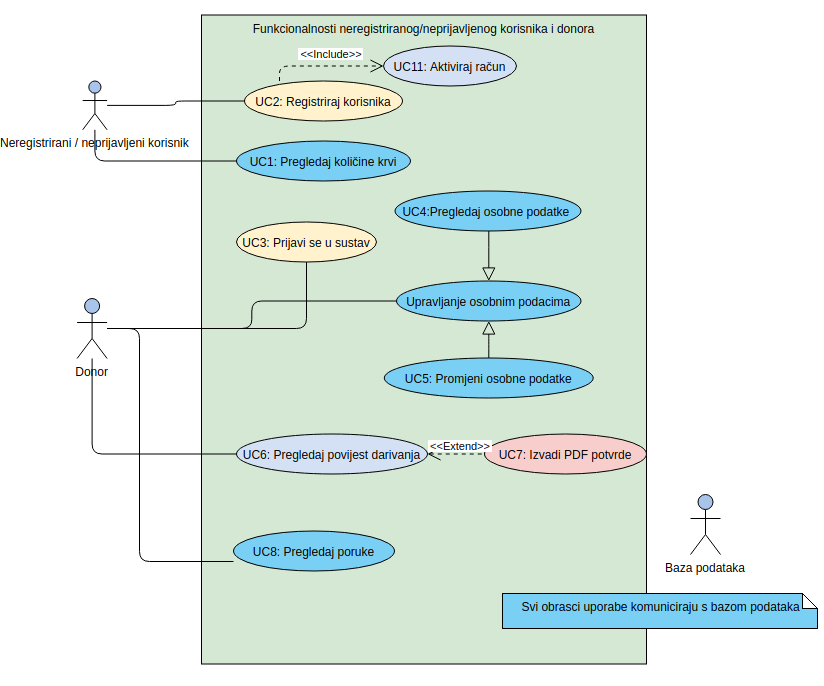
\includegraphics[scale=0.6]{dijagrami/Funkcionalnosti_korisnika_donora.png} %veličina slike u odnosu na originalnu datoteku i pozicija slike
			\centering
			\caption{Dijagram obrasca uporabe, funkcionalnost neregistriranog / neprijavljenog korisnika i donora}
			\label{fig:Funkcionalnosti_korisnika_donora}
\end{figure}

\begin{figure}[H]
			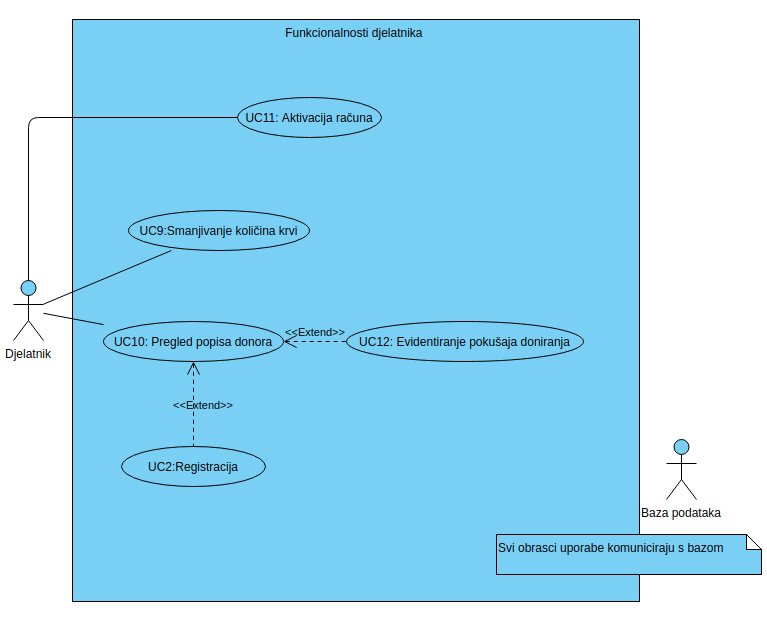
\includegraphics[scale=0.6]{dijagrami/Funkcionalnosti_djelatnika_donora.png} %veličina slike u odnosu na originalnu datoteku i pozicija slike
			\centering
			\caption{Dijagram obrasca uporabe, funkcionalnost djelatnika}
			\label{fig:Funkcionalnosti_djelatnika_donora}
\end{figure}

\begin{figure}[H]
			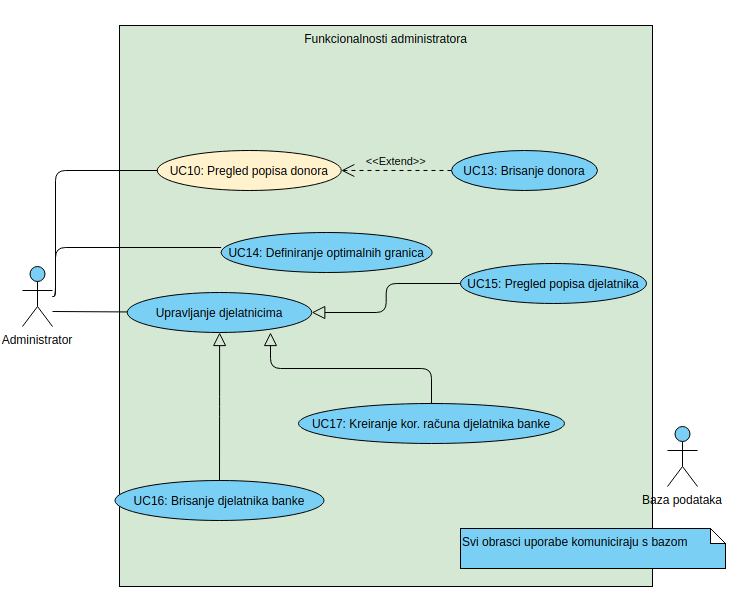
\includegraphics[scale=0.6]{dijagrami/Funkcionalnosti_admina.png} %veličina slike u odnosu na originalnu datoteku i pozicija slike
			\centering
			\caption{Dijagram obrasca uporabe, funkcionalnost administratora}
			\label{fig:Funkcionalnosti_admina}
\end{figure}

\begin{figure}[H]
			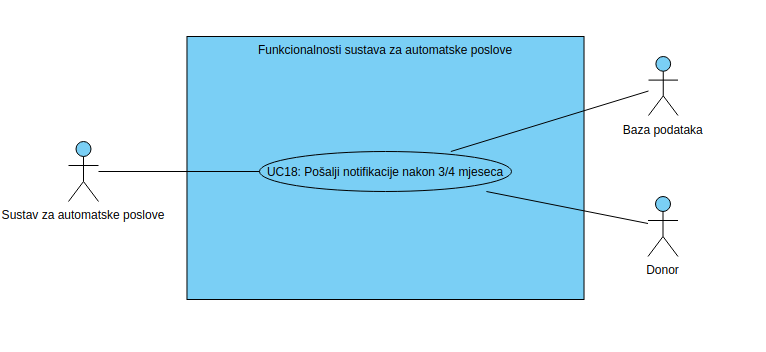
\includegraphics[scale=0.6]{dijagrami/Funkcionalnosti_auto.png} %veličina slike u odnosu na originalnu datoteku i pozicija slike
			\centering
			\caption{Dijagram obrasca uporabe, funkcionalnost sustava za automatske poslove}
			\label{fig:Funkcionalnosti_auto}
\end{figure}

\eject
		
\subsection{Sekvencijski dijagrami}

\textbf{Obrazac uporabe UC8 - Dobivanje poruke stanja zalihe krvi}

Donor, koji nema trajnu zabranu darivanja krvi, kod svakog spajanja u sustav dobiva poruku u ovisnosti o trenutnom stanju zaliha krvi. Poslužitelj dohvaća podatke iz baze podataka i prema zadanim granicama vraća jednu od tri poruka. Poruke mogu biti: stanje zaliha ispod optimalne granice; stanje zaliha je optimalno; stanje zaliha je iznad gornje optimalne granice.

\begin{figure}[H]
	\centering
	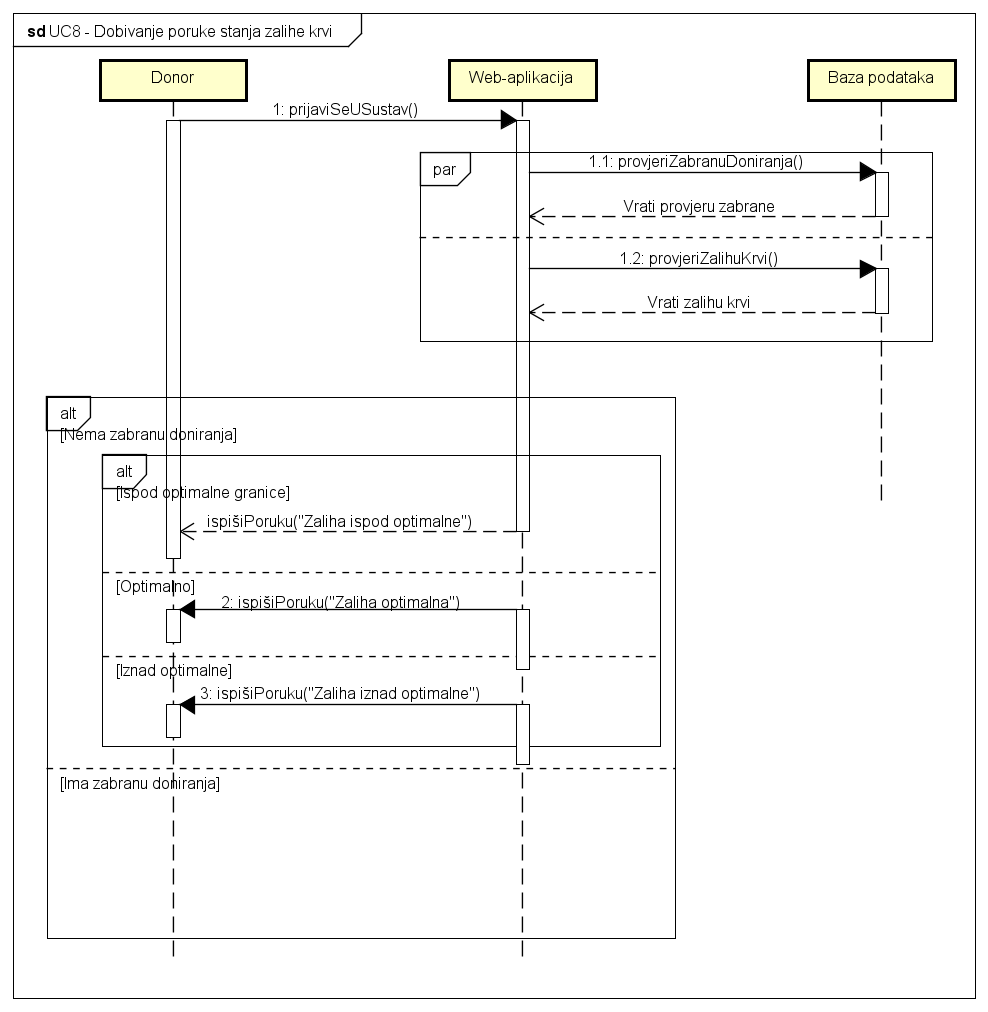
\includegraphics[width=\textwidth, scale=0.4]{dijagrami/UC8_Dobivanje poruke stanja zalihe krvi.png}
	\caption{Sekvencijski dijagram za UC8}
	\label{fig:UC8_Dobivanje poruke stanja zalihe krvi}
\end{figure}
\eject

\textbf{Obrazac uporabe UC9 - Evidentiranje "potrošnje" krvi}

Djelatnik banke može evidentirati "potrošnju" krvi odnosno slanje određenog broja jedinica krvi u vanjsku instituciju. U bazi podataka se smanjuje količina određene vrste krvi i ako se prešla donja granica šalje se mail djelatniku.

\begin{figure}[H]
	\centering
	\includegraphics[width=\textwidth, scale=0.4]{dijagrami/UC9_Evidentiranje_potrošnje_ krvi.png}
	\caption{Sekvencijski dijagram za UC9}
\end{figure}

\eject 
\textbf{Obrazac uporabe UC12 - Evidentiranje pokušaja doniranja}

Djelatnik banke evidentira i uspješne i neuspješne pokušaje doniranja. Na temelju zdravstvenog stanja donor može pristupiti doniranju, ali može i biti privremeno ili trajno odbijen. Baza podataka se ažurira, zapisuje se pokušaj doniranja krvi i ako je uspješan poveća se razina određene vrste krvi.

\begin{figure}[H]
	\centering
	\includegraphics[width=\textwidth]{dijagrami/UC12_Evidentiranje pokušaja doniranja.png}
	\caption{Sekvencijski dijagram za UC12}
\end{figure}
\eject

\textbf{Obrazac uporabe UC14 - Definiranje optimalnih granica}

Za svaku krvnu grupu administrator sustava definira gornju i donju granicu optimalne količine. Administratoru se prikazuju trenutne granice za pojedinu vrstu krvi. Zatim on ih on može mijenjati i promjene se spremaju i bazu podataka. Ako je prijeđena gornja granica šalje se mail djelatniku. Ako je prijeđena donja granica šalje se mail djelatniku i poruke donorima.

\begin{figure}[H]
	\centering
	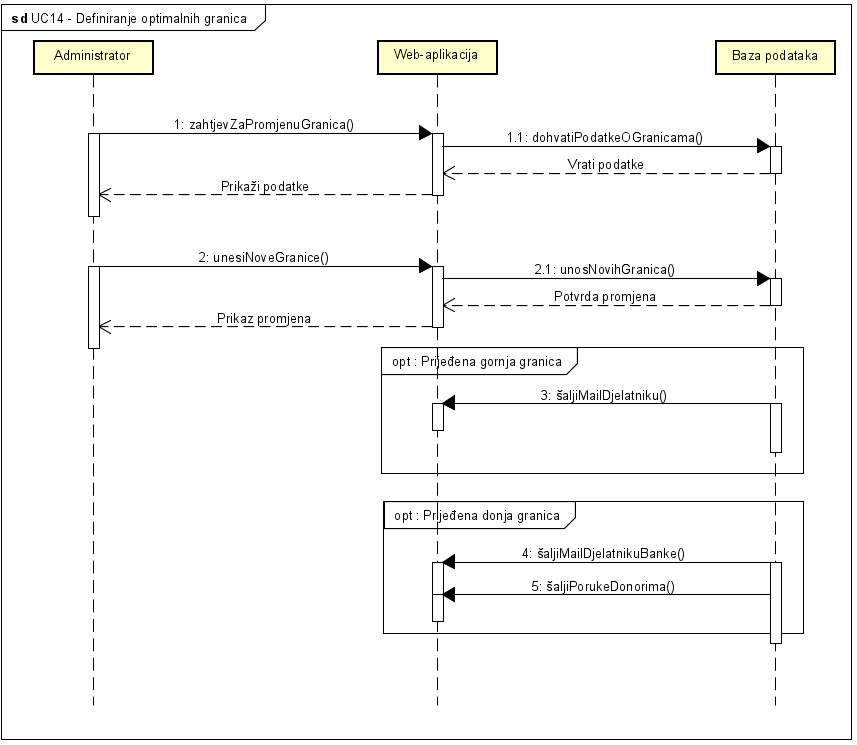
\includegraphics[width=\textwidth]{dijagrami/UC14_Definiranje optimalnih granica.png}
	\caption{Sekvencijski dijagram za UC14}
\end{figure}
\eject

\section{Ostali zahtjevi}

\begin{packed_item}
	
	\item Sustav treba biti implementiran kao web aplikacija koja je prilagođena različitim veličinama ekrana. (responsive web design)
	\item Sustavu trebaju moći pristupati tri vrste korisnika (administrator, djelatnik banke i donor). Svaki korisnik se treba ovjeravati korisničkim imenom i lozinkom.
	\item Donori trebaju imati mogućnost sami kreirati svoj korisnički račun kao i djelatnici banke u slučaju da donor sam nije napravio korisnički račun prije prvog darivanja.
	\item Administratori trebaju imati mogućnost kreiranja korisničkog računa za djelatnike banke.
	\item Novi korisnici trebaju dobiti aktivacijski link na svoj mail, donori uz aktivacijski link trebaju dobiti i donorId koji će koristiti kao korisničko ime.
	\item Prilikom aktivacije korisničkog računa, korisnici trebaju imati mogućnost odabrati svoju lozinku.
	\item Sustav treba omogućiti rad više korisnika u stvarnom vremenu.
	\item Neispravno korištenje sustava ne smije narušiti rad sustava.
	\item Korisničko sučelje treba biti intuitivno, tako da se korisnici mogu koristiti sustavom bez dodatnih uputa.
	\item Sustav treba podržavati hrvatsku abecedu pri unosu i prikazu tekstualnog sadržaja.
	\item Veza s bazom podataka mora biti zaštićena i brza.

\end{packed_item}





